\begin{figure}
  \centering
  \resizebox{\columnwidth}{!}{%
  \begin{minipage}{\textwidth} %

  %----------------------------
  % First row: NO FIXATION
  \begin{subfigure}[t]{\textwidth}
    \centering
    % Left minipage for row label (empty caption)
    \begin{minipage}[b]{0.04\textwidth}
      \caption{}
      \label{fig:dynamics:no-fixation}
    \end{minipage}
    % Six images (columns)
    \begin{minipage}[b]{0.15\textwidth}
      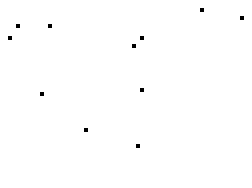
\includegraphics[width=\linewidth]{binder/binder-wse-denovo-spatial2d-explicitsite-timeseries.ipynb/binder/wse-denovo-spatial2d-explicitsite-timeseries/a=traitframes+nmut=14+rep=39a89ca6-a1b5-4b32-ae5f-f0dbb40ba027/dstream_Tbar=000504+ext=.png}
    \end{minipage}
    \begin{minipage}[b]{0.15\textwidth}
      
\includegraphics[width=\linewidth]{binder/binder-wse-denovo-spatial2d-explicitsite-timeseries.ipynb/binder/wse-denovo-spatial2d-explicitsite-timeseries/a=traitframes+nmut=14+rep=5dc8e084-0382-4d7b-9b76-6c3902ca3c1d/dstream_Tbar=000952+ext=.png}
    \end{minipage}
    \begin{minipage}[b]{0.15\textwidth}
      \includegraphics[width=\linewidth]{binder/binder-wse-denovo-spatial2d-explicitsite-timeseries.ipynb/binder/wse-denovo-spatial2d-explicitsite-timeseries/a=traitframes+nmut=14+rep=5dc8e084-0382-4d7b-9b76-6c3902ca3c1d/dstream_Tbar=001400+ext=.png}
    \end{minipage}
    \begin{minipage}[b]{0.15\textwidth}
      
\includegraphics[width=\linewidth]{binder/binder-wse-denovo-spatial2d-explicitsite-timeseries.ipynb/binder/wse-denovo-spatial2d-explicitsite-timeseries/a=traitframes+nmut=14+rep=5dc8e084-0382-4d7b-9b76-6c3902ca3c1d/dstream_Tbar=002552+ext=.png}
    \end{minipage}
    \begin{minipage}[b]{0.15\textwidth}
      
\includegraphics[width=\linewidth]{binder/binder-wse-denovo-spatial2d-explicitsite-timeseries.ipynb/binder/wse-denovo-spatial2d-explicitsite-timeseries/a=traitframes+nmut=14+rep=5dc8e084-0382-4d7b-9b76-6c3902ca3c1d/dstream_Tbar=020472+ext=.png}
    \end{minipage}
    \begin{minipage}[b]{0.15\textwidth}
      
\includegraphics[width=\linewidth]{binder/binder-wse-denovo-spatial2d-explicitsite-timeseries.ipynb/binder/wse-denovo-spatial2d-explicitsite-timeseries/a=traitframes+nmut=14+rep=5dc8e084-0382-4d7b-9b76-6c3902ca3c1d/dstream_Tbar=061424+ext=.png}
    \end{minipage}
  \end{subfigure}

  \vspace{1em} % vertical space between rows

  %----------------------------
  % Second row: FIXATION
  \begin{subfigure}[t]{\textwidth}
    \centering
    % Left minipage for row label (empty caption)
    \begin{minipage}[b]{0.05\textwidth}
      \caption{}
      \label{fig:dynamics:fixation}
    \end{minipage}
    % Six images (columns)
    \begin{minipage}[b]{0.15\textwidth}
      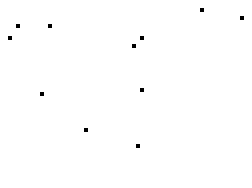
\includegraphics[width=\linewidth]{binder/binder-wse-denovo-spatial2d-explicitsite-timeseries.ipynb/binder/wse-denovo-spatial2d-explicitsite-timeseries/a=traitframes+nmut=14+rep=39a89ca6-a1b5-4b32-ae5f-f0dbb40ba027/dstream_Tbar=000504+ext=.png}
    \end{minipage}
    \begin{minipage}[b]{0.15\textwidth}
      
\includegraphics[width=\linewidth]{binder/binder-wse-denovo-spatial2d-explicitsite-timeseries.ipynb/binder/wse-denovo-spatial2d-explicitsite-timeseries/a=traitframes+nmut=14+rep=39a89ca6-a1b5-4b32-ae5f-f0dbb40ba027/dstream_Tbar=000952+ext=.png}
    \end{minipage}
    \begin{minipage}[b]{0.15\textwidth}
      \includegraphics[width=\linewidth]{binder/binder-wse-denovo-spatial2d-explicitsite-timeseries.ipynb/binder/wse-denovo-spatial2d-explicitsite-timeseries/a=traitframes+nmut=14+rep=39a89ca6-a1b5-4b32-ae5f-f0dbb40ba027/dstream_Tbar=001400+ext=.png}
    \end{minipage}
    \begin{minipage}[b]{0.15\textwidth}
      
\includegraphics[width=\linewidth]{binder/binder-wse-denovo-spatial2d-explicitsite-timeseries.ipynb/binder/wse-denovo-spatial2d-explicitsite-timeseries/a=traitframes+nmut=14+rep=39a89ca6-a1b5-4b32-ae5f-f0dbb40ba027/dstream_Tbar=002489+ext=.png}
    \end{minipage}
    \begin{minipage}[b]{0.15\textwidth}
      
\includegraphics[width=\linewidth]{binder/binder-wse-denovo-spatial2d-explicitsite-timeseries.ipynb/binder/wse-denovo-spatial2d-explicitsite-timeseries/a=traitframes+nmut=14+rep=39a89ca6-a1b5-4b32-ae5f-f0dbb40ba027/dstream_Tbar=002489+ext=.png}
    \end{minipage}
    \begin{minipage}[b]{0.15\textwidth}
      
\includegraphics[width=\linewidth]{binder/binder-wse-denovo-spatial2d-explicitsite-timeseries.ipynb/binder/wse-denovo-spatial2d-explicitsite-timeseries/a=traitframes+nmut=14+rep=39a89ca6-a1b5-4b32-ae5f-f0dbb40ba027/dstream_Tbar=002489+ext=.png}
    \end{minipage}
  \end{subfigure}

  %----------------------------
  % Timepoint labels below the bottom row:
  \begin{minipage}[c]{0.154\textwidth}
\hfill
\begin{varwidth}{\textwidth}
$T = 504$
\end{varwidth}
\hfill
  \end{minipage}
  \begin{minipage}[c]{0.154\textwidth}
\hfill
\begin{varwidth}{\textwidth}
$T = 952$
\end{varwidth}
\hfill
  \end{minipage}
  \begin{minipage}[c]{0.154\textwidth}
\hfill
\begin{varwidth}{\textwidth}
$T = 1,400$
\end{varwidth}
\hfill
  \end{minipage}
  \begin{minipage}[c]{0.154\textwidth}
\hfill
\begin{varwidth}{\textwidth}
$T = 2,552$
\end{varwidth}
\hfill
  \end{minipage}
  \begin{minipage}[c]{0.154\textwidth}
\hfill
\begin{varwidth}{\textwidth}
$T = 20,472$
\end{varwidth}
\hfill
  \end{minipage}
  \begin{minipage}[c]{0.154\textwidth}
\hfill
\begin{varwidth}{\textwidth}
$T = 61,424$
\end{varwidth}
\hfill
  \end{minipage}

  \end{minipage}%
  }%

\vspace{-2ex}

  \caption{
  \textbf{Spatiotemporal dynamics of simulated populations.}
  \footnotesize
  Snapshots show timecourse of nonmutator (white) and mutator (black) prevalence across 2D structure on WSE under limited adaptive potential.
  %, using site-explicit genome model configured to adaptive potential of 14 beneficial mutations available and mutators introduced \textit{de novo}.
  % Raster values are binary, with white pixels indicating a sampled nonmutators and black pixels indicating a sampled mutator.
  In panel \ref{fig:dynamics:no-fixation}, mutators do not reach fixation, while in panel \ref{fig:dynamics:fixation}, mutators do reach fixation.
  %  and \ref{fig:dynamics:fixation} show replicates where mutators do not, and do, reach fixation, respectively.
  Animations are provided at \url{https://hopth.ru/ej} and \url{https://hopth.ru/ek}.
  % Example timecourses for simulations with 12 and 16 beneficial mutations available can be found at \url{https://hopth.ru/el} and \url{https://hopth.ru/em}.
  }
  \label{fig:dynamics}

\vspace{-3ex}

\end{figure}
